\documentclass[11pt,twoside]{scrartcl}
\usepackage{mdas}
% \usepackage[sexy, fancy, hints]{evan}
\begin{document}
\title{Mathcounts National 2018}
% If you contribute to the handout, put your name in comment here

\author{bisv.math@gmail.com}
\org{BISV Mathcounts Club, 2020-21}
\date{\today}

\maketitle

\begin{abstract}
    Problems Copyright MATHCOUNTS, Inc. 2018. All rights reserved. 
    
    Solutions Copyright bisv.math@google.com, 2021.
\end{abstract}

\newpage
\section{Sprint}
\begin{problem}
    Alana can make a tutu in 40 minutes. Spencer takes 50\% longer. Working
    together, how many minutes does it take them to make 20 tutus?
        \begin{sketch}
        Their combined rate of work is $\frac{1}{40} + \frac{1}{60} = \frac{2.5}{60}$ tutus/minute. So together they will $\frac{20}{\frac{2.5}{60}} = \boxed{480}$ minutes.
    \end{sketch}
\end{problem}
%--------------

\begin{problem}
    What is the least positive two-digit base-three integer that is not divisible by 2? Express your answer in base three.
    \begin{sketch}
        The least positive two-digit base three number is $\boxed{10_3} = 3$, which happens to be not divisible by 2.
    \end{sketch}
\end{problem}
%--------------

\begin{problem}
    If $ k $ and $ P $ are nonzero real numbers such that the sum of $ P\% $ of $ P\% $ of $ k $ and
$ \frac{4}{5} $ of $ P\% $ of $ k $ is equal to $ P\% $ of $ k $, what is the value of $ P $?
    \begin{sketch}
        \begin{align*}
            \frac{P}{100}\cdot\cancel{\frac{P}{100}}\cdot \cancel{k} + \frac{4}{5}\cdot\cancel{\frac{P}{100}}\cdot \cancel{k} &= \cancel{\frac{P}{100}}\cdot \cancel{k}, \\
            \frac{P}{100} &= 1 - \frac{4}{5}, \\
            P &= \boxed{20}.
        \end{align*}
    \end{sketch}
\end{problem}
%--------------

\begin{problem}
    In square $ ABCD $, shown here, point $ F $ is on side $ AB $ such that
$ AF:FB =2:1 $, and point $ G $ is on side $ AD $ such that $ AG:GD = 3:1 $.
What is the ratio of the area of triangle $ AFG $ to the area of
pentagon $ FBCDG $? Express your answer as a common fraction.
    \begin{center}
        \begin{asy}
            unitsize(1cm);
            real s = 2;
            pair A, B, C, D, F, G;

            D = (0,0);
            A = (0,s);
            B = (s,s);
            C = (s,0);
            F = (2*B+A)/3;
            G = (3*D+A)/4;

            draw(A--B--C--D--cycle^^F--G);

            label("$A$", A, N);
            label("$F$", F, N);
            label("$B$", B, N);
            label("$C$", C, S);
            label("$D$", D, S);
            label("$G$", G, W);

        \end{asy}
    \end{center}
    \begin{sketch}
        Let $AB = s$. $[AFG] = \frac{1}{2}\cdot\frac{2}{3}s\cdot\frac{3}{4}s = \frac{1}{4}s^2$. Then the desired ratio is $\dfrac{\frac{1}{4}s^2}{(1-\frac{1}{4})s^2} = \boxed{\frac{1}{3}}$.
    \end{sketch}
\end{problem}
%--------------

\begin{problem}
    In the sum shown, each letter stands for a different nonzero digit. What is the three-digit number $ IKA $?
    \begin{center}
        \begin{tabular}{cccc}
            & A& P & I \\ 
            & A& P & I \\ 
            & A& P & I \\ 
            + & A& P & I \\ \hline
            & I & K & A
    
        \end{tabular}        
    \end{center}
    \begin{sketch}
        First, $4A < 10$ as otherwise we will have a 4-digit sum. So $A$ is either 1 or 2. Now looking at the last digit, we have $4I \equiv A \pmod{10}$, so $A=1$ is not possible and $A=2$, and $4I \equiv 2 \pmod{10}$, so $I$ is 3 or 8. However, since $4A + \text{carry from 2nd digit} = I$, we have $I \geq 4A$. So $I = 8$. 

        Since there is no carry from second digit addition to 3rd digit, we have $3 + 4P < 10$, and $P < 2$. Since the digits are non-zero, $P=1$, and $K=3+4\cdot1= 7$. So $IKA = \boxed{872}$.
    \end{sketch}
\end{problem}
%--------------

\begin{problem}
    If the three lines $ 3x+y=-1,x+3y=-11 $ and $ ax-2y=3 $ all intersect at one point, what is the value of $ a $?
    \begin{sketch}
        Let's find where the first two lines meet. Multiplying the first equation by 3 and subtracting the second from it, we get $8x = 8$, that is $x=1$ and $y=-4$. 
        
        Plugging this point into the third line's equation we get $a+8=3$, that is $a = \boxed{-5}$.
    \end{sketch}
\end{problem}
%--------------

\begin{problem}
    Alice and Bob play a game that begins with flipping a fair coin twice. If the coin lands heads up on both flips,Bob wins. If the coin lands heads up on only one flip, Alice wins. If the coin lands tails up on both flips, they flip two more times, and this process continues until there is a winner. What is the probability that Bob wins the game? Express your answer as a common fraction.
    \begin{sketch}
        Bob can win this flip with a probability $\frac{1}{4}$. And there is a $\frac{1}{4}$ chance that the game continues. If the game continues, Bob's probability of winning overall from that point is the same as from the starting point. Therefore we have 
        \[P(B) = \frac{1}{4} + \frac{1}{4}P(B).\]
        This gives us, $P(B) = \boxed{\frac{1}{3}}$.
    \end{sketch}
\end{problem}
%--------------

\begin{problem}
    The first and fourth terms of a geometric sequence are 4 and 9, respectively. What is the geometric mean of the second and third terms?
    \begin{sketch}
        We are given that $a=4$ and $ar^3=9$, so $r=\frac{9}{4}^{\frac{1}{3}}$. 

        The geometric mean of the second and third term is $\sqrt{ar\cdot ar^2} = a\sqrt{r^3}$.
        Plugging in the values from above, this is $4\cdot \sqrt{\frac{9}{4}} = \boxed{6}$
    \end{sketch}
\end{problem}
%--------------

\begin{problem}
    The mean, median and unique mode of a list of seven positive integers are all equal to 10. What is the greatest possible range of the list?
    \begin{sketch}
        From the given conditions, we have $\underline{?}\ \underline{?}\ \underline{?}\ \underline{10}\ \underline{?}\ \underline{?}\ \underline{?}$. Our goal is to put as small values in the spaces other than the last space. This means that the two other spaces to the immediate right of the center, we need to put 10. This gives $\underline{?}\ \underline{?}\ \underline{?}\ \underline{10}\ \underline{10}\ \underline{10}\ \underline{?}$.

        Now, we need to have the smallest values in the first 3 spaces, but to preserve unique mode we can not repeat an element 3 times. This leads to: $\underline{1}\ \underline{1}\ \underline{2}\ \underline{10}\ \underline{10}\ \underline{10}\ \underline{?}$. 

        To preserve the mean as 10, the last digit is $10 + 2\cdot (10-1) + (10-2) = 36$, and the range is $36 - 1 = \boxed{35}$
    \end{sketch}
\end{problem}
%--------------

\begin{problem}
    What is the probability that a randomly chosen positive integer factor of 11,088 is not divisible by any perfect square greater than 1? Express your answer as a common fraction.
    \begin{sketch}
        First, $11,088 = 2^4\cdot 3^2 \cdot 7 \cdot 11$. The square free factors can have 0 or 1 of each of the 4 prime factors. Therefore, the desired probability is:
        \[\frac{2\cdot2\cdot\cancel{2}\cdot\cancel{2}}{5\cdot3\cdot\cancel{2}\cdot\cancel{2}} = \boxed{\frac{4}{15}}.\]
    \end{sketch}
\end{problem}
%--------------

\begin{problem}
    The graph of the line $ 2x+3y=8 $ intersects the $ x $-axis at $ A $ and intersects the $ y $-axis at $ B $. Points $ A,B $ and $ O(0,0) $ form right triangle $ ABO $. If triangle $ ABO $ is dilated about the origin by a scale factor of $ -\frac{3}{4} $, what is the area of dilated triangle $ A'B'O' $?
    \begin{sketch}
        $A = (4,0)$, and $B = (0,\frac{8}{3})$, so $[ABO] = \frac{1}{2}\cdot4\cdot\frac{8}{3} = \frac{16}{3}$. $[A'B'O'] = \big(\frac{3}{4}\big)^2 \cdot \frac{16}{3} = \boxed{3}$
    \end{sketch}
\end{problem}
%--------------

\begin{problem}
    Rudy has a basket of perfectly cylindrical cookies of varying sizes. He has seven cookies of radius 3 inches, eight cookies of radius 2 inches and seven cookies of radius 1 inch. All cookies are 0.25 inch thick. Rudy splits the cookies into 3 groups such that each group's cookies have the same total volume. If all the cookies remain whole, what is the fewest possible number of cookies in any group?
    \begin{sketch}
        Since the cookies, remain whole, $h$ of the cookies is not going to change. Let's consider the $\frac{V}{\pi \cdot h}$. Total $\frac{V}{\pi \cdot h} = 7\cdot3^2 + 8 \cdot 2^2 + 7 \cdot 1^2 = 112$. In each basket, this value will be $\frac{1}{3}\cdot 112 = 34$. 
        
        That is, if there are $a,b,c$ of each in a basket we will have $9a + 4b + c = 34.$ We can find the values of $(a,b,c)$ that satisfy this is $(3,1,3), (2,4,0), (2, 3, 4), (1,6,1), (1, 4, 5), (0,8,2), (0,7,6)$. Of these, the smallest number is for the combination $(2,4,0)$, which is $\boxed{6}$.

        Note: We need not have considered all the possibilities because the smallest volume would include either 3 or 2 of $a$. (The reason we can not immediately assume 3, is that by giving a little more to $b+c$, we can have more $c$ rolled up in $b$.)
    \end{sketch}
\end{problem}
%--------------

\begin{problem}
    What common fraction is equivalent to the sum shown?
    \[ \frac{1}{2018+1} + \frac{1}{2018^2+2018+1} + \frac{1}{2018^4+2(2018^3)+2(2018^2)+2018} \]
    \begin{sketch}
        First, note that $x^2 + x + 1 = \frac{x^3-1}{x-1}$.
        Next, factorize $x^4 + 2x^3 + 2x^2 + x$,
        \begin{align*}
            &= x^4 + x^3+x^2 + x^3 + x^2 + x, \\
            &= x^2(x^2+x+1) + x(x^2+x+1), \\
            &= (x^2+x)(x^2+x+1), \\
            &= x(x+1)(x^2+x+1).
        \end{align*}     
        So the given fraction (with 2018 replaced by $x$) can be written as,
        \begin{align*}
            &\frac{1}{x+1} + \frac{x-1}{x^3-1} + \frac{x-1}{x(x+1)(x^3-1)}, \\
            &= \frac{x(x^3-1)+x(x+1)(x-1)+(x-1)}{x(x+1)(x^3-1)}, \\
            &= \frac{x(x^3-1) + x^3 - \cancel{x} + \cancel{x} - 1}{x(x+1)(x^3-1)}, \\
            &= \frac{(x^3-1)(x+1)}{x(x+1)(x^3-1)}, \\
            &= \frac{1}{x}.
        \end{align*}
        And, so our answer is $\boxed{\frac{1}{2018}}$
    \end{sketch}
\end{problem}
%--------------

\begin{problem}
    Jenny rolls four standard six-sided dice, each with faces numbered one through six.What is the probability that there is at least one pair of dice whose top faces sum to 12? Express your answer as a common fraction.
    \begin{sketch}
        We do complementary counting. Probability that there is at least one pair such that \ldots is
        \begin{align*}
            &1 - P(0) - P(1), \\
            &= 1 - \Big(\frac{5}{6}\Big)^4 - \binom{4}{1}\cdot\frac{1}{6}\cdot\Big(\frac{5}{6}\Big)^3, \\
            &= \frac{6^4-5^4-4\cdot5^3}{6^4}, \\
            &= \boxed{\frac{19}{144}}.
        \end{align*}
    \end{sketch}
\end{problem}
%--------------

\begin{problem}
    The faces of two cubes are painted so that the colors of the six faces on each cube are red,orange, yellow, green, blue and violet, in some random order. What is the probability that the two cubes can be rotated so that their colorings are identical? Express your answer as a common fraction.
    \begin{sketch}
        \textbf{Solution 1. }
        Orient the cubes so that the red face is on top the probability that they have the same color opposite the red face is $\dfrac{1}{5}$. Then for the remaining 4 colors there are 4 rotations that is ${\dfrac{4!}{4}}$ arrangements, so $\dfrac{1}{6}$ probability of getting the right colors on the side. Finally, the final probability that the 2 cubes can be rotated so that their colorings are identical is $\dfrac{1}{5}\cdot\dfrac{1}{6} = \dfrac{1}{30}.$

        \textbf{Solution 2. }
        Essentially, we need to know how many rotational symmetries are there for a cube. That is how many cube orientation can be arrived from one by rotating across its various lines of symmetries. Let's count this:
        \begin{itemize}
            \item Diagonal line of symmetry. There are 4 of these for each pair of diagonally opposite vertices. And we can rotate by $120^\circ$ and $240^\circ$. So total of 8.
            \item Center of opposite faces line of symmetry. There are 3 of these for each pair of opposite faces. And we can rotate by $90^\circ$, $180^\circ$, and $270^\circ$. So total of 9.
            \item Center of opposite edges line of symmetry. There are 6 of these for each opposite pair of edges. We can rotate by $180^\circ$. So total of 6.
            \item Identity. Let's not forget the original orientation.   
        \end{itemize}
        So we have a total of $8 + 9 + 6 + 1 = 24$ rotational symmetries.
\begin{remark}
    You can see an animation of these rotations at: \\
    \url{https://ubpdqnmathematica.wordpress.com/2011/02/06/rotational-symmetries-of-cube/}.

    Also, there are videos in You Tube demonstrating this. Search for ``Rotational Symmetry of Cube.''
\end{remark}        
    Therefore, we have $\frac{6!}{24} = 30$ unique possibilities of cube accounting for rotational symmetries. And the probability that the second cube is the same as the first (accounting for rotational symmetry) is 
        $\boxed{\frac{1}{30}}$.
    \end{sketch}
\end{problem}
%--------------

\begin{problem}
    The bases of the right hexagonal prism shown are regular hexagons with sides of length 4 inches. Space diagonals $ AD' $ and $ CF' $ intersect at a right angle. What is the length of edge $ EE' $? Express your answer in simplest radical form.

    \begin{center}
        \begin{asy}
        import three;        
        currentprojection=orthographic(3, -50, 20);

        unitsize(1cm);
        real s = 4;

        pair A, A1, B, B1, C, C1, D, D1, E, E1, F, F1;

        F = (0,0);
        E = (s, 0);
        A = rotate(120, F)*E;
        D = rotate(-120, E)*F;
        C = rotate(-120, D)*E;
        B = rotate(-120, C)*D;

        draw((F.x, F.y, 0)--(E.x, E.y, 0)--(D.x, D.y, 0)--(C.x, C.y, 0)--(B.x, B.y, 0)--(A.x, A.y, 0)--cycle);
        draw((F.x, F.y, -s)--(E.x, E.y, -s)--(D.x, D.y, -s)--(C.x, C.y, -s)--(B.x, B.y, -s)--(A.x, A.y, -s)--cycle);
        draw((F.x, F.y, 0)--(F.x, F.y, -s)^^(E.x, E.y, 0)--(E.x, E.y, -s)^^(D.x, D.y, 0)--(D.x, D.y, -s)^^(C.x, C.y, 0)--(C.x, C.y, -s)^^(B.x, B.y, 0)--(B.x, B.y, -s)^^(A.x, A.y, 0)--(A.x, A.y, -s));

        draw((A.x, A.y, 0)--(D.x, D.y, -s)^^(C.x, C.y, 0)--(F.x, F.y, -s), dashed);

        label("$A$", (A.x, A.y, 0), N);
        label("$B$", (B.x, B.y, 0), N);
        label("$C$", (C.x, C.y, 0), N);
        label("$D$", (D.x, D.y, 0), N);
        label("$E$", (E.x, E.y, 0), N);
        label("$F$", (F.x, F.y, 0), N);

        label("$A'$", (A.x, A.y, -s), S);
        label("$B'$", (B.x, B.y, -s), S);
        label("$C'$", (C.x, C.y, -s), S);
        label("$D'$", (D.x, D.y, -s), S);
        label("$E'$", (E.x, E.y, -s), S);
        label("$F'$", (F.x, F.y, -s), S);

        \end{asy}
    \end{center}
    
    \begin{sketch}
        Consider the crossection $ACD'F'$. Since it's a rectangle and we are given that its diagonals intersect at right angle, we know that it is square, implying $AF' = AC$. 
        
        Now if we look at the $\triangle ABC$, we have $AB = BC = s$, and $\angle ABC = 120^\circ$. From this, we can calculate $AC = \sqrt{3}s$. We could use law of consine directly to do this. Or we can drop an altitude from $C$ to $AF$, say $H$, and use the fact that $\triangle CFH$ is a 30-60-90 triangle to know that $CH = \frac{\sqrt{3}}{2}s$, $HF = \frac{1}{2}s$, and $AF = s + HF = \frac{3}{2}s$. Then from Pythagoras on $\triangle CHA$, we have $AC^2 = CH^2 + AH^2 = \frac{3}{4}s^2 + \frac{9}{4}s^2 = 3s^2$.
        
        Now looking at the $\triangle AFF'$, we have from Pythagoras on it, $AF'^2 = s^2 + FF'^2$. Plugging in value of $AF' = AC$ from above, we get $FF' = \sqrt{2}s = \boxed{4\sqrt{2}}.$
    \end{sketch}
\end{problem}
%--------------

\begin{problem}
    In a card game, Nora draws cards at random, without replacement,from a deck of 21 cards. Twenty of the cards are numbered 1 through 20, and the other card is marked ``Joker.'' Nora keeps all of the cards she draws before she draws the Joker. What is the probability that the cards Nora keeps include exactly four prime-numbered cards? Express your answer as a common fraction.
    \begin{sketch}
        We can simply ignore all cards other than the prime numbered cards and the Joker as drawing or not drawing them makes no difference. In other words we can formulate this as drawing cards from a pack of 8 prime numbered cards and 1 joker such that we draw a prime numbered card the first 4 times and Joker in the fifth. With this formulation, its easy to see that the probability is
        \[\frac{8}{9} \cdot \frac{7}{8} \cdot\frac{6}{7} \cdot\frac{5}{6} \cdot\frac{1}{5} = \boxed{\frac{1}{9}}. \] 
    \end{sketch}
\end{problem}
%--------------

\begin{problem}
    How many assignments of digits $ A, B, C $ and $ D $ exist such that the four-digit numbers $ ABCD_6 $ and $ ABCD_{10} $ are both divisible by 5?
    \begin{sketch}
        \textbf{Solution 1. }
        $D$ must be 0 or 5, then pick any $B$ and $C$ between 0 and 5, inclusive. Then, there is exactly 1 choice of $A$ from $(1, 2, 3, 4, 5)$ that makes $ABCD$ base 6 divisible by 5. Thus, we have $2\cdot6\cdot6\cdot1=\boxed{72}$ possibilities. 

        \textbf{Solution 2. }
        First, since $ABCD_6$ is a valid number, we have $$ 0 \leq A,B,C,D \leq 5, \text{ and } A \not = 0.$$

        Second, $5 \mid ABCD_{10}$ tells us that $$D \equiv 0\pmod 5, \text{ that is } D \in \{0, 5\}.$$

        Next, from $5 \mid ABCD_{6}$, we have 
        \begin{align*}
            A \cdot 6^3 + B \cdot 6^2 + C \cdot 6 + D \equiv 0\pmod 5, \\
            A \cdot 1^3 + 1 \cdot 1^2 + C \cdot 1 + 0 \equiv 0\pmod 5, \\
            A + B + C \equiv 0 \pmod 5. 
        \end{align*} 
        From here, we could simply do casework on $A$. Alernatively, we do casework on $A+B+C$:
        \begin{itemize}
            \item $A+B+C=5$: If we have $A, B, C \geq 0$, from Stars and Bars, we have $\binom{7}{2} = 21$ ways. Of which $\binom{6}{1} =6$ have $A=0$. Therefore, for this case we have $21-6 = 15$ ways.
            \item $A+B+C=10$: With $A, B, C \geq 0$, from Stars and Bars, we have $\binom{12}{2} = 66$ ways. However, in this are included the cases where 
            \begin{itemize}
                \item One of them is $ \geq 6$. Let's say $A \geq 6$. Let's have $A' = A - 6 /geq 0$, and $A' + B + C = 4$. This can happen in $\binom{6}{2} = 15$ ways and since any of the three can be the one $ \geq 6$ we have a total of $3\cdot15 = 45$ ways.
                \item $A = 0$. There is only 1 way, $B=5, C=5$. 
            \end{itemize}
            In summary, for this case we have $66 - 45 - 1 = 20$ ways.
            \item $A+B+C=15$: There is only 1 way: $A=5, B=5, C=5$.
        \end{itemize}
        So in total we have $15 + 20 + 1 = 36$ ways, and for each way $D$ can be 0 or 5, so final answer is $2 \cdot 36 = \boxed{72}$
    \end{sketch}
\end{problem}
%--------------

\begin{problem}
    In the figure, $ ABCD $ is a square with area $ 1024 \text{ cm}^2 $. $ P $ is the midpoint of side $ CD $. $ Q $ is the midpoint of segment $ BP $. $ R $ is the midpoint of segment $ AQ $. $ S $ is the midpoint of segment $ DR $. $ T $ is the midpoint of segment $ CS $. $ T $ is also the intersection of segments $ BP $ and $ CS $. What is the area of quadrilateral $ QRST $?
    \begin{center}
        \begin{asy}
            unitsize(1cm);
            real s = 5;
            pair A, B, C, D, P, Q, R, S, T;

            A = (s,s);
            B = (0,s);
            C = (0,0);
            D = (s,0);

            P = (C+D)/2;
            Q = (B+P)/2;
            R = (A+Q)/2;
            S = (D+R)/2;
            T = (C+S)/2;

            draw(A--B--C--D--cycle);
            draw(B--P^^A--Q^^D--R^^C--S);

            label("$A$", A, NE);
            label("$B$", B, NW);
            label("$C$", C, SW);
            label("$D$", D, SE);
            label("$P$", P, SE);
            label("$Q$", Q, SW);
            label("$R$", R, NW);
            label("$S$", S, NE);
            label("$T$", T, N);

        \end{asy}
    \end{center}
    \begin{sketch}
        First, 
        \[[QRST] = [ABCD] - [\triangle BCP] - [\triangle ABQ] - [\triangle ADR] - [\triangle CDS] + [\triangle CPT].\]
        \begin{center}
            \begin{asy}
                unitsize(1cm);
                real s = 5;
                pair A, B, C, D, P, Q, R, S, T;
    
                A = (s,s);
                B = (0,s);
                C = (0,0);
                D = (s,0);
    
                P = (C+D)/2;
                Q = (B+P)/2;
                R = (A+Q)/2;
                S = (D+R)/2;
                T = (C+S)/2;
    
                draw(A--B--C--D--cycle);
                draw(B--P^^A--Q^^D--R^^C--S);
                
                draw("$\frac{1}{2}s$", Q--(Q.x,B.y), E, blue+dashed);
                draw("$\frac{1}{4}s$", R--(R.x,B.y), E, blue+dashed);
                draw("$\frac{3}{4}s$", R--(R.x,0), W, purple+dashed);
                draw("$\frac{3}{8}s$", S--(S.x,0), W, purple+dashed);
                draw("$\frac{3}{16}s$", T--(T.x,0), W, purple+dashed);

                draw("$(\frac{1}{2}+\frac{1}{4}=\frac{3}{4})s$", Q--(s, Q.y), N, red+dashed);
                draw("$\frac{3}{8}s$", R--(s, R.y), N, red+dashed);

                label("$A$", A, NE);
                label("$B$", B, NW);
                label("$C$", C, SW);
                label("$D$", D, SE);
                label("$P$", P, SE);
                label("$Q$", Q, SW);
                label("$R$", R, NW);
                label("$S$", S, NE);
                label("$T$", T, N);
    
            \end{asy}
        \end{center}
        From the above figure,
        \begin{itemize}
            \item $[\triangle BCP] = \frac{1}{2} \cdot s \cdot \frac{1}{2}s = \frac{1}{4}s^2.$
            \item $[\triangle ABQ] = \frac{1}{2} \cdot \frac{1}{2}s \cdot s = \frac{1}{4}s^2.$
            \item $[\triangle ADR] = \frac{1}{2} \cdot \frac{3}{8}s \cdot s = \frac{3}{16}s^2.$
            \item $[\triangle CDS] = \frac{1}{2} \cdot \frac{3}{8}s \cdot s = \frac{3}{16}s^2.$
            \item $[\triangle CPT] = \frac{1}{2} \cdot \frac{3}{16}s \cdot \frac{1}{2}s = \frac{3}{64}s^2.$
        \end{itemize}
        Putting it all together,
        \begin{align*}
            [QRST] &= s^2 - 2\cdot \frac{1}{4}s^2 - 2 \cdot \frac{3}{16}s^2 + \frac{3}{64}s^2, \\
            &= \Big(1 - \frac{1}{2} - \frac{6}{16} + \frac{3}{64}\Big)s^2, \\
            &= \frac{64 - 32 - 24 + 3}{64}s^2, \\
            &= \frac{11}{64}\cdot 1024, \\
            &= \boxed{176}.
        \end{align*}
    \end{sketch}
\end{problem}
%--------------

\begin{problem}
    Vanessa tosses a fair coin eight times. If the coin lands heads up, she steps 1 meter west. If the coin lands tails up, she steps 1 meter north. What is the probability that Vanessa ends a distance of at most 6 meters away from her starting position? Express your answer as a common fraction.
    \begin{sketch}
        First, there are $2^8 = 256$ ways she can take the steps, each equally likely. Let's count how many of these ways lands her further than 6 meters away. These are:
        \begin{itemize}
            \item $(0,8),(-8,0)$: $2$ ways.
            \item $(-1,7),(-7,1)$: $2\cdot\binom{8}{1} = 16$ ways.
            \item $(-2,6),(-6,2)$: $2\cdot\binom{8}{2} = 56$ ways.
        \end{itemize}
        So thenumber of ways, she ends up within a distance of 6 is $256 - 2 - 16 - 56 = 182$, and the desired probability is $\dfrac{182}{256} = \boxed{\frac{91}{128}}$


    \end{sketch}
\end{problem}
%--------------

\begin{problem}
    What is the greatest integer that is less than or equal to $ \dfrac{3^{19} + 2^{19}}{3^{15} + 2^{15}} $?
    \begin{sketch}
        \begin{align*}
            \frac{3^{19} + 2^{19}}{3^{15} + 2^{15}} &= \frac{3^4\cdot3^{15}+3^4\cdot2^{15}-3^4\cdot2^{15}+2^{19}}{3^{15} + 2^{15}}, \\
            &= 3^4 - \frac{3^4\cdot2^{15}-2^{19}}{3^{15} + 2^{15}}, \\
            &= 3^4 - \frac{2^{15}\cdot65}{3^{15} + 2^{15}}, \\
            &= 3^4 - \frac{2^{15}\cdot(2^6+1)}{3^{15} + 2^{15}}, \\
            &= 3^4 - \frac{2^{21} + 2^{15}}{3^{15} + 2^{15}}.
        \end{align*}

        Since $2^3 < 3^2$, we have $2^{21} < 3^{14}$. Therefore,
        \[ 0 < \frac{2^{21} + 2^{15}}{3^{15} + 2^{15}} < 1. \]
        And our answer is $\boxed{80}$
    \end{sketch}
\end{problem}
%--------------

\begin{problem}
    The polynomials $ x^3+5x^2-69x+180 $ and $ x^3+8x^2-36x+144 $ share a common
factor of the form $ x + a $. What is the value of $ a $?
    \begin{sketch}
        Since $-a$ is the root of both the polynomials, we have 
        \begin{align*}
            -a^3 + 5a^2 + 69a + 180 &= 0, \\
            -a^3 + 8a^2 + 36a + 144 &= 0, \\
            \cline{1-2}
            3a^2 -33a - 36 &= 0, \\
            a^2 - 11a - 12 &= 0, \\
            (a - 12)(a + 1) &= 0.
        \end{align*}
        Plugging $a=-1$ in the equations don't work but $a=12$ does. Therefore, the answer is $\boxed{12}.$
    \end{sketch}
\end{problem}
%--------------

\begin{problem}
    Xena and Yolanda toss an unfair coin that lands heads up $ 75\% $ of the time. If the coin lands heads up, Xena gets a point. Otherwise, Yolanda gets a point. The game ends when one player has a two-point lead over the other, and the player with the two-point lead is the winner. What is the probability that Xena wins the game? Express your answer as a common fraction.
    \begin{sketch}
        Let $x$ be Xena's points and $y$ be Yolanda's points. Then we can think of the problem in terms of $x-y$ and the different values for $x-y$ and its transitions are shown in the diagram below:

        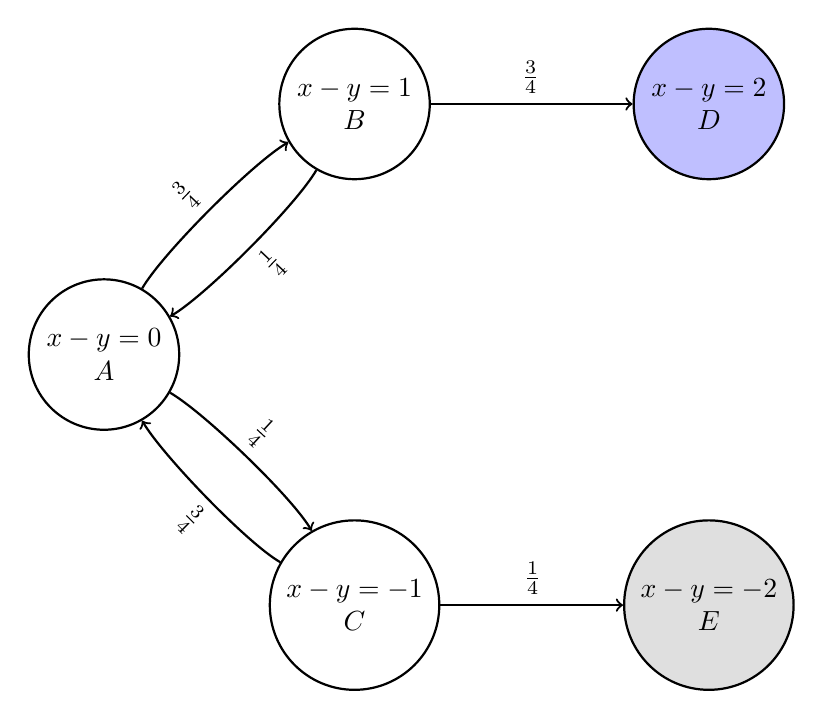
\begin{tikzpicture}[node distance={45mm}, thick, main/.style = {draw, circle}] 
            \node[main, align=center] (1) {$x-y=0$\\$A$}; 
            \node[main, align=center] (2) [above right of=1] {$x-y=1$\\$B$}; 
            \node[main, align=center] (3) [below right of=1] {$x-y=-1$\\$C$}; 
            \node[main, align=center] (4) [right of=2, fill=blue!25] {$x-y=2$\\$D$}; 
            \node[main, align=center] (5) [right of=3, fill=gray!25] {$x-y=-2$\\$E$}; 
            \draw[->] (1) to [out=60, in=210, looseness=.5] node[midway, above right, sloped, pos=0.4] {$\frac{3}{4}$}(2); 
            \draw[->] (2) to [out=240, in=30, looseness=.5] node[midway, below left, sloped, pos=0.4] {$\frac{1}{4}$}(1); 
            \draw[->] (1) to [out=-30, in=120, looseness=.5] node[midway, above right, sloped, pos=0.4] {$\frac{1}{4}$}(3); 
            \draw[->] (3) to [out=150, in=-60, looseness=.5] node[midway, below left, sloped, pos=0.4] {$\frac{3}{4}$}(1); 

            \draw[->] (2) to node[midway, above right, sloped, pos=0.4] {$\frac{3}{4}$}(4); 
            % \draw[->] (4) to [out=195, in=-15, looseness=.5] node[midway, above right, sloped, pos=0.6] {+2}(2); 

            \draw[->] (3) to  node[midway, above right, sloped, pos=0.4] {$\frac{1}{4}$}(5); 
            % \draw[->] (5) to [out=195, in=-15, looseness=.5] node[midway, above right, sloped, pos=0.6] {+2}(3); 
            % \draw[->] (6) -- node[midway, above right, sloped, pos=1] {+1} (4); 
        \end{tikzpicture} 

        Let $P_A, P_B, P_C$ denote the chances of Xena winning given that we are currently in state $A, B, C$, respectively.

        Then from the above diagram, we can see that:
        \begin{align*}
            P_A = \frac{3}{4}P_B + \frac{1}{4}P_C, \\
            P_B = \frac{3}{4} + \frac{1}{4}P_A, \\
            P_C = \frac{3}{4} P_A.
        \end{align*}
        We can solve the above equations to get $P_B = \frac{39}{40}$, and 
        $$P_A = \frac{12}{13}\cdot\frac{39}{40} = \boxed{\frac{9}{10}}.$$
    \end{sketch}
\end{problem}
%--------------

\begin{problem}
    The figure shows isosceles right triangle $ ABC $ with $ AC=BC=16 $ units. Triangle $ ABD $ is constructed within triangle $ ABC $ with vertex $ D $ on side $ AC $ and $ AD = 4 $ units. Point $ E $ is drawn on side $ AB $ to form isosceles right triangle $ ADE $. A series of isosceles right triangles is constructed within triangle $ ABD $, such that the hypotenuse of each lies on side $ AB $, the 90-degree vertex of each lies on segment $ BD $, and each shares a vertex with the preceding triangle in the series, as shown. What is the combined area of the series of isosceles right triangles within triangle $ ABD $? Express your answer as a common fraction.    

    \begin{center}
        \begin{asy}
            import olympiad;

            unitsize(0.5cm);
            pair A, B, C, D, E, F, G, H, I, J, K, L;

            A = (0,0);
            B = (16, 0);
            C = (8, 8);
            D = (2, 2);
            E = (4, 0);

            F = (E.x+(3/4)*2, (3/4)*2);
            G = (E.x+(3/4)*4, 0);

            H = (G.x+(3/4)*(3/4)*2, (3/4)*(3/4)*2);
            I = (G.x+(3/4)*(3/4)*4, 0);

            J = (I.x+(3/4)*(3/4)*(3/4)*2, (3/4)*(3/4)*(3/4)*2);
            K = (I.x+(3/4)*(3/4)*(3/4)*4, 0);

            L = (K.x+(3/4)*(3/4)*(3/4)*(3/4)*2, (3/4)*(3/4)*(3/4)*(3/4)*2);

            draw(A--B--C--cycle);
            draw(B--D--E--F--G--H--I--J--K--L);

            draw(rightanglemark(A, C, B));
            draw(rightanglemark(A, D, E));
            draw(rightanglemark(E, F, G));
            draw(rightanglemark(G, H, I));
            draw(rightanglemark(I, J, K));

            label("$A$", A, SW);
            label("$B$", B, SE);
            label("$C$", C, N);
            label("$D$", D, NW);
            label("$E$", E, S);
            label("$F$", F, N);
            label("$G$", G, S);
            label("$16$", B--C, NE);
            label("$4$", A--D, NW);

            label("$\ldots$", (L.x+0.4, L.y/2));
        \end{asy}
    \end{center}
    \begin{sketch}
        Since $ \triangle DEF \sim \triangle FGH$, $\frac{EF}{DE} = \frac{GH}{FG}$, and because the triangles are isoceles this means $\frac{EF}{AD} = \frac{GH}{EF}$. That is each successive triangle is a dilation of the previous one by a constant factor, say $k$. Therefore, the total area of these triangles is
        \begin{align*}
            & (1 + k^2 + k^4 + k^{16} + \ldots)[\triangle ADE], \\
            &= \frac{1}{1-k^2}\cdot \frac{1}{2} \cdot 4 \cdot 4, \\
            &= \frac{1}{1-k^2} \cdot 8.
        \end{align*} 
        We need to find $k$.

        \begin{center}
            \begin{asy}
                import olympiad;
    
                unitsize(0.5cm);
                pair A, B, C, D, E, F, G, H, I, J, K, L;
    
                A = (0,0);
                B = (16, 0);
                C = (8, 8);
                D = (2, 2);
                E = (4, 0);
    
                F = (E.x+(3/4)*2, (3/4)*2);
                G = (E.x+(3/4)*4, 0);
    
                H = (G.x+(3/4)*(3/4)*2, (3/4)*(3/4)*2);
                I = (G.x+(3/4)*(3/4)*4, 0);
    
                J = (I.x+(3/4)*(3/4)*(3/4)*2, (3/4)*(3/4)*(3/4)*2);
                K = (I.x+(3/4)*(3/4)*(3/4)*4, 0);
    
                L = (K.x+(3/4)*(3/4)*(3/4)*(3/4)*2, (3/4)*(3/4)*(3/4)*(3/4)*2);
    
                draw(A--B--C--cycle);
                draw(B--D--E--F--G--H--I--J--K--L);
    
                draw(rightanglemark(A, C, B));
                draw(rightanglemark(A, D, E));
                draw(rightanglemark(E, F, G));
                draw(rightanglemark(G, H, I));
                draw(rightanglemark(I, J, K));
    
                label("$A$", A, SW);
                label("$B$", B, SE);
                label("$C$", C, N);
                label("$D$", D, NW);
                label("$E$", E, S);
                label("$F$", F, N);
                label("$G$", G, S);
                label("$H$", H, NE);
                label("$16$", B--C, NE);
                label("$4$", A--D, NW);
    
                label("$\ldots$", (L.x+0.4, L.y/2));

                label("$x$", E--F, NW);

                Label L = Label("$4\sqrt{2}$", align=(0,0), position=MidPoint, filltype=Fill(white));
                draw((A.x,-1) -- (E.x,-1), L=L, arrow=Arrows(), bar=Bars);   
                L = Label("$16\sqrt{2}$", align=(0,0), position=MidPoint, filltype=Fill(white));
                draw((A.x,-1.5) -- (B.x,-1.5), L=L, arrow=Arrows(), bar=Bars);   

            \end{asy}
        \end{center}
        We have $$k = \frac{x}{4} = \frac{16\sqrt{2}-4\sqrt{2}}{16\sqrt2} = \frac{3}{4}.$$
        Plugging this in our previous expression, we get $ \dfrac{1}{1-\frac{9}{16}}\cdot 8 = \boxed{\frac{128}{7}}$
    \end{sketch}
\end{problem}
%--------------

\begin{problem}
    If $ a_1,a_2,a_3,a_4,a_5 $ is an increasing geometric sequence of real numbers such that
$ a_3=1 $ and $ a_1+a_5=10 $, then the value of $ a_4 $ can be expressed in simplest radical
form as $ \sqrt{a} + \sqrt{b} $.What is the value of $ a+b $?
    \begin{sketch}
        Let the numbers be $\frac{1}{r^2}, \frac{1}{r},1,r,r^2$. We need to find $r = ?$. We have
        \begin{align*}
            r^2 + \frac{1}{r^2} &= 10, \\
            r^4 - 10r^2 + 1 &= 0, \\
            (r^2)^2 - 10r^2 + 1 &= 0.
        \end{align*}
        This yields
        \begin{align*}
            r^2 &= \frac{10 \pm \sqrt{96}}{2}, \\
            &= 5 \pm 2\sqrt{6}.
        \end{align*}
        Also, 
        \begin{align*}
            r &= \sqrt{a} + \sqrt{b}, \\
            r^2 &= a + b + 2\sqrt{ab}.
        \end{align*} 

        From the above 2 equations, we have $a + b = \boxed{5}$
    \end{sketch}
\end{problem}
%--------------

\begin{problem}
    The rational number one-seventh can be written as a repeating base ten decimal as $ 0.\overline{142857} $. The same rational number can be written as a repeating ``decimal'' in base nine. What is the sum, in base nine, of the first hundred digits to the right of the ``decimal'' point?
    \begin{sketch}
        First, we can work out the repeating ``decimal'' in other bases, similar to how we do in base 10. Say a fraction $\frac{a}{b}$ can be written as a repeating ``decimal'' in base $b$ with $n$ being the length of the repeat, then similar to base 10 we get
        \[ ([1\underbrace{0\ldots0}_{n \text{ length}}]_b -1) \cdot \frac{a}{b} = \text{repetend}.\]
        For $b=9$ and $\frac{1}{7}$, this means:
        \[ [\underbrace{8\ldots8}_{n \text{ length}}]_b \cdot \frac{1}{7} = \text{repetend}.\]

        What that means is that for the smallest $n$ such that $8\ldots8_9$ of length $n$ is divisible by 7, the reptend will be the quotient on dividing $8\ldots8_9$ by 7.
        
        From here, we have 2 approaches.

        \paragraph{Method 1 - Base 9 Division} We can divide $8\ldots8_9$ by 7 in base 9, till we get a divisible length. Since division in other bases is not a common operation, we work through the details here. To divide in base $b$, it helps to write out the multiplication table in base $b$ first. Here is the multiplication table in base $9$ for $7$:
        \begin{align*}
            \begin{array}{*3c}
                7 \times 1 = 7_9 & 7 \times 4 = 31_9 & 7 \times 7 = 54_9 \\
                7 \times 2 = 15_9 & 7 \times 5 = 38_9 & 7 \times 8 = 62_9 \\
                7 \times 3 = 23_9 & 7 \times 6 = 46_9 &
            \end{array}
        \end{align*} 
        We can do long division in base $b$ same as in base 10 - we just need to take the products from the correct multiplication table. Here is the long divison of $8\ldots8_9$ by 7 in base 9.
        \begin{align*}
            \renewcommand\arraystretch{.75}\renewcommand\arraycolsep{3pt}
            \begin{array}{r@{\hskip\arraycolsep}c@{\hskip\arraycolsep}*4r} % n=5=2+4
              &&1&2&5\\
              \cline{2-6} %n=8
             7&\Big)&8&8&8&\ldots \\
              &&7&& \\
              \cline{3-6}\\
              &&1&8& \\
              &&1&5& \\
              \cline{3-6}\\
              &&&3&8 \\
              &&&3&8 \\
              \cline{4-6}\\
            \end{array}
          \end{align*}
          We see that in step 3 there is no reminder, so we have $888_7 \div 7 = 125$.

          \paragraph{Method 2} If we are not comfortable with division in base 9, we can also work this out using regular too. First, note that $8 \equiv 1 \pmod{7}$ and $9 \equiv 2 \pmod{7}$. Therefore,
          \begin{align*}
              8 &\equiv 1 \pmod{7}, \\
              88 &\equiv 1 \cdot 2 + 1 \equiv 3 \pmod{7}, \\
              888 &\equiv 1 \cdot 2^2 + 1 \cdot 2 + 1 \equiv 0 \pmod{7}.
          \end{align*} 
          Now that we know that $888_9$ is divisible by 7, we can do
          \[\frac{888_7}{7} = \frac{728_{10}}{7} = 104_{10} = 125_9.\]

          We have found that
          \[\Big(\frac{1}{7}\Big)_9 = 0.\overline{125}.\]


          Therefore, the sum of the first hundred digits to the the right of the decimal is 
          \begin{align*}
              33_{10}\cdot(1+2+5)_{10} + 1 &= 33_{10}\cdot(8)_{10} + 1_{10}, \\
              &= 36_{9}\cdot(8)_{9} + 1_9, \\
              &= 323_9 + 1_9, \\
              &= \boxed{324_9}.  
          \end{align*}
          
          In case $36_{9}\cdot(8)_{9} = 323_9$ is not obvious, here are the steps:
          \begin{align*}
              6 \times 8 &= 53_9, \text{carry of 5}, \\
              3 \times 8 + 5 &= 26_9 + 5_9 = 32_9.
          \end{align*}
          Alternatively, we could do the operations in base 10 and then convert it back to base 9. $33_{10}\cdot(1+2+5)+1=265_{10}$, and we can convert back to base 9 using:
          \begin{align*}
              265 &= 29 \cdot 9 + \underline{4}, \\
              29 &= \underline{3} \cdot 9 + \underline{2}.
          \end{align*}
          Yielding, $265_{10} = 324_9$.
    \end{sketch}
\end{problem}
%--------------

\begin{problem}
    An equilateral triangle is divided into 16 congruent equilateral triangles, half of which are shaded, and point $ P $ lies at a vertex as shown. If a random line passing through point $ P $ is drawn,what is the probability that the line divides the total shaded area exactly in half? Express your answer as a common fraction.
    \begin{center}
        \begin{asy}
            unitsize(1.25cm);
            real s = 4, h = sqrt(3)*s/2;
            pair P = (3*s/8, h/4);

            for (int i = 0; i < 2; ++i) {
                real x1, x2, y;
                x1 = i*s/4+s/8;
                x2 = s - x1;
                y = (2*i+1)*h/4;

                for (int j = 0; j < 3 - 2*i; ++j) {
                    real xj = x1 + j*s/4;

                    filldraw((xj, y)--(xj+s/8,y-h/4)--(xj+s/4,y)--(xj+s/8,y+h/4)--cycle, gray(0.5), black);
                }
                draw((x1,y)--(x2,y));
            }
            draw((0,0)--(s,0)--(s/2,h)--cycle^^(s/4,h/2)--(3*s/4,h/2));
            dot(P, red);
            label("$P$", P, N);
        \end{asy}
    \end{center}

    \begin{sketch}
        From the diagram, we can see that the line has to be between $l_1$ and $l_2$. If it moves further anti clockwise form $l_1$, the right side starts getting more of the shaded area. And if it moves further clockwise from $l_2$, the upper side starts getting more of the shaded area.

        \begin{center}
            \begin{asy}
                pair l1_1, l1_2, l2_1, l2_2;

                unitsize(1.25cm);
                real s = 4, h = sqrt(3)*s/2;
                pair P = (3*s/8, h/4);
    
                l1_1 = P + ((s/4,0)-P)*1.40;
                l1_2 = P + ((5*s/8, 3*h/4)-P)*1.25;

                l2_1 = P + ((0,0)-P)*1.25;
                l2_2 = P + ((3*s/4, h/2)-P)*1.25;

                for (int i = 0; i < 2; ++i) {
                    real x1, x2, y;
                    x1 = i*s/4+s/8;
                    x2 = s - x1;
                    y = (2*i+1)*h/4;
    
                    for (int j = 0; j < 3 - 2*i; ++j) {
                        real xj = x1 + j*s/4;
    
                        filldraw((xj, y)--(xj+s/8,y-h/4)--(xj+s/4,y)--(xj+s/8,y+h/4)--cycle, gray(0.7), black);
                    }
                    draw((x1,y)--(x2,y));
                }
                draw((0,0)--(s,0)--(s/2,h)--cycle^^(s/4,h/2)--(3*s/4,h/2));
                dot(P, red);
                label("$P$", P, N);

                draw(Label("$l_1$", EndPoint), l1_1--l1_2, blue);
                draw(Label("$l_2$", EndPoint), l2_1--l2_2, blue);
                markangle("$\alpha$",l2_2,P,l1_2,red);
                markangle("$\beta$",(7*s/8, h/4),P,l2_2,red);
            \end{asy}
        \end{center}
        So we need to find the angle $\alpha$ between the two lines. We have $ \alpha + \beta = 60^\circ$ as the triangles are equilateral. Also, $\beta = 30^\circ$ by symmetry (or as $l_2$ is the median of the equilateral triangle of size 4). Therefore, $\alpha = 30^\circ$ and the desired probability is $\dfrac{30}{180} = \boxed{\frac{1}{6}}.$
    \end{sketch}
\end{problem}
%--------------

\begin{problem}
    How many six-digit positive integers containing six distinct nonzero digits are divisible by 99?
    \begin{sketch}
        Let the six-digit integer be $\overline{abcdef}$. Then divisibility by 9 implies:
        \[a +b + c + d + e +f \equiv 0 \mod 9.\]
        And divisibility by 11 implies:
        \[(a+c+e)-(b+d+f) \equiv 0 \mod 11.\]
        Let's do casework on $(a+c+e)-(b+d+f)$.
        \begin{itemize}
            \item $(a+c+e)-(b+d+f) = 0$: Then $(a+c+e)=(b+d+f) \equiv 0 \mod 9$. Looking at the cases for $(a+c+e)=(b+d+f)$, we have:
            \begin{itemize}
                \item $(a+c+e)=(b+d+f)=9$. There is no cases where where we can have distinct digits satisfying this.
                \item $(a+c+e)=(b+d+f)=18$. There are three pairs:
                \begin{align*}
                    \begin{array}{c|c}
                        a+c+e=18 & b+d+f=18 \\ \hline
                        1,8,9 & 5,6,7 \\
                        2,7,9 & 4,6,8 \\
                        3,7,8 & 4,5,9 \\
                    \end{array}   
                \end{align*}
                Since each of the above can be reversed between the first column and second column, we have $2 \cdot 3 = 6$ ways. 
                \item 27 or higher sums cannot be achieved with distinct digits.
            \end{itemize}
            \item $(a+c+e)-(b+d+f) = \pm 11$: (we will consider only $+11$ and then multiply by 2 to get the $-11$ cases by symmetry). Plugging in $(b+d+f) = (a+c+e)-11$ into the divisibility condition above for 9 yields:
            \begin{align*}
                2(a+c+e) - 11 &\equiv 0 \mod 9, \\
                2(a+c+e) &\equiv 2 \mod 9, \\
                (a+c+e) &\equiv 1 \mod 9.
            \end{align*}
            We now do casework on subcases for $a+c+e$:
            \begin{itemize}
                \item $a+c+e = 10$: $b+d+f =1$ is not possible.
                \item $a+c+e = 19$: $b+d+f =8$. This yields the following 5 pairs:
                \begin{align*}
                    \begin{array}{c|c}
                        a+c+e=19 & b+d+f=8 \\ \hline
                        2,8,9 & 1,3,4 \\
                        3,7,9 & 1,2,5 \\
                        4,6,9 & 1,2,5 \\
                        4,7,8 & 1,2,5 \\
                        5,6,8 & 1,3,4
                    \end{array}   
                \end{align*}
            \end{itemize}
            Multiplying by 2 to account for the earlier mention symmetry, we have $2\cdot5=10$ ways.
            \item $(a+c+e)-(b+d+f) = \pm 22$: Not possible as with unique digits the largest possible difference is $(9+8+7)-(3+2+1) = 18$. 
        \end{itemize}
        Therefore we have a total of $10+6 = 16$ combinations of $(a,c,e)$ and $(b,d,f)$. Within each such combination we can permute the digits. So the total possibilities are $ 16 \cdot 3! \cdot 3! = \boxed{576}.$
    \end{sketch}
\end{problem}
%--------------

\begin{problem}
    Isosceles trapezoid $ ABCD $ has parallel bases $ AB $ and $ CD $. Point $ E $ is the intersection of diagonals $ AC $ and $ BD $.The height of the trapezoid is $ 20 $ cm. The area of triangle $ ADE $ is 75 cm. If bases $ AB $ and $ CD $ have integer lengths with $ AB< CD $, what is the sum of all possible values of $ AB $?

    \begin{center}
        \begin{asy}
            unitsize(0.25cm);
            pair A, B, C, D, E;
        
            D= (0,0);
            C= (18,0);
            A= (4, 20);
            B = (12,20);
        
            E = intersectionpoint((D--B), (A--C));
        
            draw(D--C--B--A--cycle^^D--B^^C--A);
            label("$D$", D, SW);
            label("$C$", C, SE);
            label("$B$", B, NE);
            label("$A$", A, NW);
            label("$E$", E, S);  
            
            // filltype = background color
            Label L = Label("$20$", align=(0,0), position=MidPoint, filltype=Fill(white));
            draw((C.x+4,C.y) -- (C.x+4,C.y+20), L=L, arrow=Arrows(), bar=Bars);   

        \end{asy}
    \end{center}
    \begin{sketch}
        Let $AB=a$, and $DC=c$. First, let's get some bounds on $a$. 

        \begin{center}
        \begin{asy}
            unitsize(0.25cm);
            pair A, B, C, D, E;
        
            D= (0,0);
            C= (18,0);
            A= (4, 20);
            B = (12,20);
        
            E = intersectionpoint((D--B), (A--C));
        
            fill (A--E--D--cycle, gray(0.9));

            draw(D--C--B--A--cycle^^D--B^^C--A);
            label("$D$", D, SW);
            label("$C$", C, SE);
            label("$B$", B, NE);
            label("$A$", A, NW);
            label("$E$", E, S);  
            
            // filltype = background color
            Label L = Label("$20$", align=(0,0), position=MidPoint, filltype=Fill(white));
            draw((C.x+4,C.y) -- (C.x+4,C.y+20), L=L, arrow=Arrows(), bar=Bars);   

            label("$75$", (A+E+D)/3);
            label("$a$", A--B, N, blue);
            label("$c$", D--C, N, blue);
            L = Label("$\frac{c}{c+a}\cdot20$", align=(0,0), position=MidPoint, filltype=Fill(white));
            draw((C.x+8,C.y) -- (C.x+8,E.y), L=L, arrow=Arrows(), bar=Bars, blue);   

        \end{asy}
        \end{center}
        We have $[ABD] = \frac{1}{2} \cdot 20 \cdot a > 75$, implying $a \geq 8$. 

        Next, we know that $a < c$; when $a = c$, we have $[ABD] = \frac{1}{2} \cdot \frac{a}{2} \cdot 20 = 75, a = 15$. Therefore, $ a < 15 $. So we have $$ 8 \leq a \leq 14. $$

        Now, considering the area of $\triangle ADC$, we get:
        \begin{align*}
            75 + \frac{1}{2} \frac{c}{c+a}\cdot20 \cdot c &= \frac{1}{2} \cdot 20 \cdot c, \\
            75 (c + a) + 10 c^2 &= 10c \cdot (c + a), \\
            75 (c + a) + \cancel{10 c^2} &= \cancel{10 c^2} + 10 ac, \\
            c &= \frac{75a}{10a - 75}, \\
            c &= \frac{15a}{2a - 15}.
        \end{align*}
        Since, $c$ is an integer, this means $2a - 15 \mid 15a$. In the range $ 8 \leq a \leq 14$, $8,9,10,12$ satisfy this. And so the sum of possible values of $a$ is $8+9+10+12=\boxed{39}.$
    \end{sketch}
\end{problem}
%--------------

\begin{problem}
    In the figure, $ AB=DA=5 $ units, $ AC=DE =4 $ units and $ BC=AE =3 $ units. Point $ C $ lies on segment $ AD $. It is possible to move triangle $ ABC $ onto triangle $ DAE $ by reflecting triangle $ ABC $ across a line $ m $, and then translating the image in a direction parallel to $ m $. Line $ m $ divides triangle $ ABC $ into two regions. What is the ratio of the area of the smaller region to the area of the larger region? Express your answer as a common fraction.
    \begin{center}
        \begin{asy}
            unitsize(0.75cm);
            pair A, B, C, D, E;
    
            real xt = -3/2, yt = -1/2;
    
            A = (0,4);
            C = (0,0);
            D = (0, -1);
            B = (3,0);
            E = (-12/5,11/5);    
    
            draw(A--C--B--cycle--E--D--C);
            
    
            label("$A$", A, N);
            label("$B$", B, SE);
            label("$C$", C, SE);
            label("$D$", D, S);
            label("$E$", E, N);
        \end{asy}
    \end{center}
    \begin{sketch}
        First, let's note down which reflected point slides on to which point after the final transform. Since $\triangle ACB \cong \triangle DEA$, $A' \to D, C' \to E, B' \to A$, where $A',B',C'$ are the reflections of $A, B, C$ (before the translation).

        Next, the fact that the reflected line can be slid onto $\triangle AED$ means that the lines $AB', EC', DA'$ are all parallel to $m$.

        This leads to a diagram such as the one below:

        \begin{center}
            \begin{asy}
                import cse5;
                unitsize(1cm);
                pair A, B, C, D, E, Cp, Bp, Ap, Cp2, Bp2, Ap2, H;
        
                real xt = -3/2, yt = -1/2;
        
                A = (0,4);
                C = (0,0);
                D = (0, -1);
                B = (3,0);
                E = (-12/5,11/5);
        
                real dEA, dED;
        
                dEA = distance(E, A);
                dED = distance(E, D);
        
                Cp = (E.x-xt, E.y - yt);
                Bp = (A.x-xt, A.y-yt);
                Ap = (D.x-xt, D.y-yt);
        
        
                Cp2 = (C + Cp)/2;
                Bp2 = (B + Bp)/2;
                Ap2 = (A + Ap)/2;
        
                //H = extension(A, Bp, D, Ap);
        
                draw(Ap--Bp--Cp--cycle, blue);
        
                draw(Ap2--Bp2--Cp2);
                draw(C--Cp^^A--Ap^^B--Bp, green);

                draw(A--Bp^^E--Cp^^D--Ap, purple);
                draw(Ap--B,purple+dashed);
        
                dot(Cp2);
                dot(Bp2);
                dot(Ap2);
        
                //dot(H, red);
        
                draw(A--C--B--cycle--E--D--C);
                
                //label ("Bp2: " + format(Bp2.x) + ", " + format(Bp2.y), (-2,8));
                //label ("H: " + format(H.x) + ", " + format(H.y), (-2,7));
        
                    dot((0, 3/2), red);
                    dot((3/2, 2), red);
        
                label("$A$", A, N);
                label("$A'$", Ap, S);
                label("$B$", B, SE);
                label("$B'$", Bp, N);
                label("$C$", C, SE);
                label("$D$", D, S);
                label("$C'$", Cp, N);
                label("$E$", E, N);
        
                label("$P$", (0, 3/2), SE);
                label("$Q$", (3/2, 2), SE);
            \end{asy}

            \textbf{Explanation of Diagram} In the diagram above, $PQ$ is the line $m$, the green lines are the reflection lines (each perpendicular to $m$). The purple lines show the translation of the reflected points. And the purple dashed line $A'B$ is the reflection of the translation line $AB'$.

        \end{center}

        Now $AA' \perp m$ and $BB' \perp m$ since $A', B'$ are reflections over $m$. Now, from the translation condition we have $AB' \parallel m$, which also means $A'B \parallel m$ and it is the reflection of the other. Therefore, we have $AB'BA'$ is a rectangle. This implies that $Q$, the point of intersection of $m$ with $AB$ is midpoint of $AB$ as well as $A'B'$.
        
        Let $P = m \cap AD$. We have $AB' \parallel PQ \parallel DA'$ and since $Q$ is the midpoint of $A'B'$, $P$ is the midpoint of $AD$.
        
        To summarize, we have:
        \[ AQ = \frac{1}{2} AB, \quad AP = \frac{1}{2} AD. \]

        Therefore, 
        \[\frac{[APQ]}{[ACB]} = \frac{AP \cdot AQ}{AC \cdot AB} = \frac{\frac{5}{2}\cdot\frac{5}{2}}{4 \cdot 5} = \frac{5}{16}.\]

        And the desired answer is 
        \[\frac{[APQ]}{[ACB]-[APQ]} = \frac{\frac{5}{16}}{1-\frac{5}{16}} = \boxed{\frac{5}{11}}. \]        
    \end{sketch}
\end{problem}
%--------------
\newpage
\section{Target}
\begin{problem}
    What is the slope of the line containing the point $ (5,-2) $ that is perpendicular to the line $ 2x+3y=4 $? Express your answer as a common fraction.
    \begin{sketch}
        $-\dfrac{1}{-\frac{2}{3}} = \boxed{\frac{3}{2}}$
    \end{sketch}
\end{problem}
%--------------

\begin{problem}
    A list contains 20 numbers. For each positive integer $ n $ from 1 to 20, the $ n $th number in the list is either $ \frac{1}{2}n $ or $ 2n $. If the mean of the numbers in the list is exactly 12 and the product of the numbers is $ P $, what is the greatest possible value of $ \frac{P}{20!} $?
    \begin{sketch}
        Let $a$ be the number of $\frac{1}{2}n$, and $b$ be the number of $2n$. Then $\frac{P}{20!} = 2^{b-a}$. Therefore, we want to maximize $b-a$ with $b+a=20$ while keeping the mean of numbers to be be 12; instead of mean equal to 12, we can use total equal to 240, as it is easier to work with.

        For any choice of $b$, the least total is obtained when the first $b$ elements are $2n$, and the remaining are $\frac{1}{2}n$; let's call this $f(b)$.

        We can do some trial and error. 
        \begin{align*}
            f(14) = \frac{1}{2}(15+\cdots+20) + 2 \cdot \frac{14\cdot15}{2} = 262.5, \\
            f(13) = \frac{1}{2}(14+\cdots+20) + 2 \cdot \frac{13\cdot14}{2} = 241.5, \\
            f(12) = \frac{1}{2}(13+\cdots+20) + 2 \cdot \frac{12\cdot13}{2} = 222.
        \end{align*}

        From the above, we can see $13$ is not possible, but $12$ could be.

        Let's see if we can swap out some elements that are $2n$ in the lowest configuration for $12$. Since the current total has only a deficit of $18$, we need to stay close to $12$. In fact, $f(13)=141.5$ suggests that we could finagle around it. Let's convert $13, 15$ to $2n$ and change $12$ to $\frac{1}{2}n$. The net change in total is $(13+15-12)\cdot1.5 = 24$, which overshot by 6, that we can adjust by changing 4 to $\frac{1}{2}n$. Now the total change is $(15+13-12-4)\cdot1.5=18$, exactly what we needed. And our $b$ is unchanged at 12.

        Then 
        \[ \frac{P}{20!} = 2^{12-8} = \boxed{16}. \]

    \end{sketch}
\end{problem}
%--------------

\begin{problem}
    If $ p\oplus q=\sqrt{p^2+q^2} $ and $ p \ominus q=\sqrt{p^2-q^2} $, what is the value of
\[(1\oplus2\oplus3\oplus4\oplus5\oplus6\oplus7\oplus9\oplus10) \ominus(1\oplus2\oplus3\oplus4\oplus5\oplus6\oplus7\oplus8\oplus9)? \]
    \begin{sketch}
        Notice that 8 is missing from the first part and 10 from the second part. Let $x = 1\oplus2\oplus3\oplus4\oplus5\oplus6\oplus7\oplus9$, that is all the terms minus the two missing one.

        Then our expression is same as 
        \begin{align*}
            & \sqrt{x^2+100} \ominus \sqrt{x^2+64}, \\
            &= \sqrt{x^2 + 100 -x^2 - 64}, \\
            &= \sqrt{36} = \boxed{6}.
        \end{align*}
    \end{sketch}
\end{problem}
%--------------

\begin{problem}
    When completely filled in, each cell in the five-by-five array shown will contain integers an integer so that the sum of the integers in each contiguous two-by-two square block of cells is positive. What is the greatest possible number of negative integers in the array?
    \begin{center}
        \begin{asy}
            unitsize(0.5cm);

            for (int i = 0; i < 6; ++i) {
                draw((i,0)--(i,5)^^(0,i)--(5,i));
            }
        \end{asy}
    \end{center}
    \begin{sketch}
        Note that a cell can dominate upto 8 of its neighbors, this leads to a configuration as shown below:

        \begin{center}
            \begin{asy}
                unitsize(1cm);
                
                for (int i = 0; i < 6; ++i) {
                    draw((i,0)--(i,5)^^(0,i)--(5,i));
                }
                for (int i = 0; i < 5; ++i)
                for (int j = 0; j < 5; ++j) {
                    string val = "$-1$";

                    if ((i == 1 || i == 3) && (j == 1 || j == 3)) {
                        val = "$+100$";
                    }
                    label(val,(i+0.5,j+0.5));
                }
            \end{asy}
        \end{center}
    
        The number of negative cells in the above configuration is $25 - 4 = \boxed{21}$
    \end{sketch}
\end{problem}
%--------------

\begin{problem}
    In equation $ AB+CD=EFG $, each letter represents a different digit. What is the greatest possible value of the three-digit number $ EFG $?
    \begin{sketch}
        The greatest value would be got by setting $A=9, B=8$, which sets $E=1,F=7$. The next largest option for $G = 6$, which is possible with $B=4,C=2$. Therefore, the largest value for $EFG$ is $\boxed{176}$
    \end{sketch}
\end{problem}
%--------------

\begin{problem}
    Micaela randomly chooses a real number $ w $ between -20 and 20. What is the probability that the graphs of $ x -|y| = w $ and $ x^2 + y^2 = 50 $ intersect at exactly two points? Express your answer as a decimal to the nearest hundredth.
    \begin{sketch}
        As seen in the diagram below, $-\sqrt{50} \leq w < \sqrt{50}$ satisfy the criteria.
        Therefore, the probability is $\dfrac{2\cdot\sqrt{50}}{40} = \boxed{0.35}$.
        
        \begin{center}
            \begin{asy}
                unitsize(0.25cm);
                
                draw(circle((0,0),5));
                draw((-8,0)--(8,0));

                draw((10,5)--(5,0)--(10,-5), red);

                draw(Label("$w = \sqrt{50}$", BeginPoint), (13,8)--(5,0)--(13,-8), red);
                draw(Label("$w = -\sqrt{50}$", BeginPoint), (3,8)--(-5,0)--(3,-8), blue);

                dot((0,0));

            \end{asy}
        \end{center}

    \end{sketch}
\end{problem}
%--------------

\begin{problem}
    A 4-up number is defined as a positive integer that is divisible by neither 2 nor 3 and does not have 2 or 3 as any of its digits. How many numbers from 400 to 600, inclusive, are 4-up numbers?
    \begin{sketch}
        First, we can count the numbers that are divisible by 2 or 3. We have divisible by 2 as 101, by 3 as 67, and by 6 as 34. So $101 + 67 - 34 = 134$ numbers in this range are divisible by 2 or 3. 

        Then we count the numbers that have a 2 or 3 in their digit and are not divisible by 2 or 3. One way of doing that is to list all the odd numbers with 2 or 3 as a digit, then strike out the ones divisible by 3.
        This way we get:
        \begin{align*}
            403,413, \\
            421, \cancel{423}, 425, 427, \cancel{429}, \\
            431, 433, \cancel{435}, 437, 439, \\
            443, \cancel{453}, 463, 473, \cancel{483}, 493, \\
            503,\cancel{513}, \\
            521, 523, \cancel{525}, 527, 529, \\
            \cancel{531}, 533, 535, \cancel{537}, 539, \\
            \cancel{543}, 553, 563, \cancel{573}, 583, 593. \\
        \end{align*}
        We have $25$ numbers in the above list. So the number of valid 4-up numbers is $201 - 134 -25 = \boxed{42}$
    \end{sketch}
\end{problem}
%--------------

\begin{problem}
    Shane cuts out a paper circle of radius 7 cm. He then draws two perpendicular chords, as shown, with one a distance of 1 cm from the center and the other 3 cm from the center. Next, Shane folds the bottom of the circle up along the first chord and then folds the left side of the folded circle to the right along the second chord. If the folded arcs intersect at a point P, as shown, what is the distance from the vertex of the right angle formed by the folds to P? Express your answer in simplest radical form.

    \begin{center}
        \begin{asy}
            unitsize(0.35cm);

            picture p1, p2;
            pair O, O1, O2, A1, A2, B1, B2, P, Q, M;
            pair ip[];

            path c, a1, a2;

            O = (0, 0);
            O1 = (-6, 0);
            O2 = (0, -2);

            M = (-3,-1);

            c = circle(O, 7);

            ip = intersectionpoints(c, (-3,-7)--(-3,7));
            A1 = ip[0];
            B1 = ip[1];

            ip = intersectionpoints(c, (-7,-1)--(7,-1));
            A2 = ip[0];
            B2 = ip[1];

            Q = intersectionpoints(circle(O1, 7), M--B2)[0];

            a1 = arc(O1, Q, A1);

            P = intersectionpoints(a1,circle(O2, 7))[0];
            a2 = arc(O2, B2, P);

            draw(p1, c);
            dot(p1, O);
            // dot(p1, A1, red);
            // dot(p1, A2, blue);

            draw(p1, A1--B1^^A2--B2, dashed);

            draw(p2, arc(O, B2, A1)--M--cycle^^a1^^a2);
            draw(p2, M--P, dashed);
            dot(p2, P);
            dot(p2, O);

            label(p2, "$P$", P, NE);
            label(p2, "?", M--P, SE);

            add(p1);
            add(shift(15*right)*p2);
        \end{asy}
    \end{center}
    \begin{sketch}
        From the $\triangle O_1OO_2$, we have $M$ is the midpoint of $O_1O_2$ because the two lines of folding are the midlines of those sides. 

        \begin{center}
            \begin{asy}
                unitsize(0.5cm);
    
                picture p1, p2;
                pair O, O1, O2, A1, A2, B1, B2, P, Q, M;
                pair ip[];
    
                path c, a1, a2;
    
                O = (0, 0);
                O1 = (-6, 0);
                O2 = (0, -2);
    
                M = (-3,-1);
    
                c = circle(O, 7);
    
                ip = intersectionpoints(c, (-3,-7)--(-3,7));
                A1 = ip[0];
                B1 = ip[1];
    
                ip = intersectionpoints(c, (-7,-1)--(7,-1));
                A2 = ip[0];
                B2 = ip[1];
    
                Q = intersectionpoints(circle(O1, 7), M--B2)[0];
    
                a1 = arc(O1, Q, A1);
    
                P = intersectionpoints(a1,circle(O2, 7))[0];
                a2 = arc(O2, B2, P);
    
                draw(p1, c);
                dot(p1, O);
                // dot(p1, A1, red);
                // dot(p1, A2, blue);
    
                draw(p1, A1--B1^^A2--B2, dashed);
    
                draw(p1, arc(O1, B1, A1)^^arc(O2, B2, A2), red+opacity(0.5));
                dot(p1, O1, red);
                dot(p1, O2, red);

                draw(P--O1--O2--cycle^^P--M, blue);
                draw(p1, O1--O--O2, green);

                label(p1, "$P$", P, NE);
                label(p1, "$M$", M, SW);
                label(p1, "$O_1$", O1, SW);
                label(p1, "$O_2$", O2, SE);
                label(p1, "$O$", O, NE);


                add(p1);
                // add(shift(15*right)*p2);
            \end{asy}
        \end{center}

        Therefore, $\triangle PO_1O_2$ is an isoceles triangle with $PM$ as its median. We have
        \[O_2M^2 = 3^2 + 1^2 = 10.\]
        Then 
        \[PM = \sqrt{PO_2^2 - O_2M^2} = \sqrt{7^2 - 10} = \boxed{\sqrt{39}}.\]
    \end{sketch}
\end{problem}
%--------------


\clearpage

\section{Solution Sketches}
\makehints

\end{document}